\documentclass{article}
\usepackage[utf8]{inputenc}
\usepackage{graphicx}
\usepackage{pgfplots}

\title{Complex Social Networks: Lab 1}
\author{Francesc Roy Campderrós \& Juan Pablo Royo Sales}
\date{September 2020}

\begin{document}

\maketitle
\newpage

\section{Introduction}

\noindent In this project we are going to model one fictitious network using the Watts Strogatz model and another one using the Erdös-Rényi model. Then we are going to analyze some of its topological properties.\newline

\noindent For the WS network we are going to plot  the  clustering  coefficient  and  the  average shortest-path (both normalized) as a function of the parameter p.\newline

\noindent For the ER network we are going to plot the  average  shortest-path  length  as  a  function  of  the  network  size.\newline

\section{Implementation and results}

\noindent \underline{WS Network:} The implementation was done repeating the same experiment one hundred times and averaging. \newline

\begin{center}
    

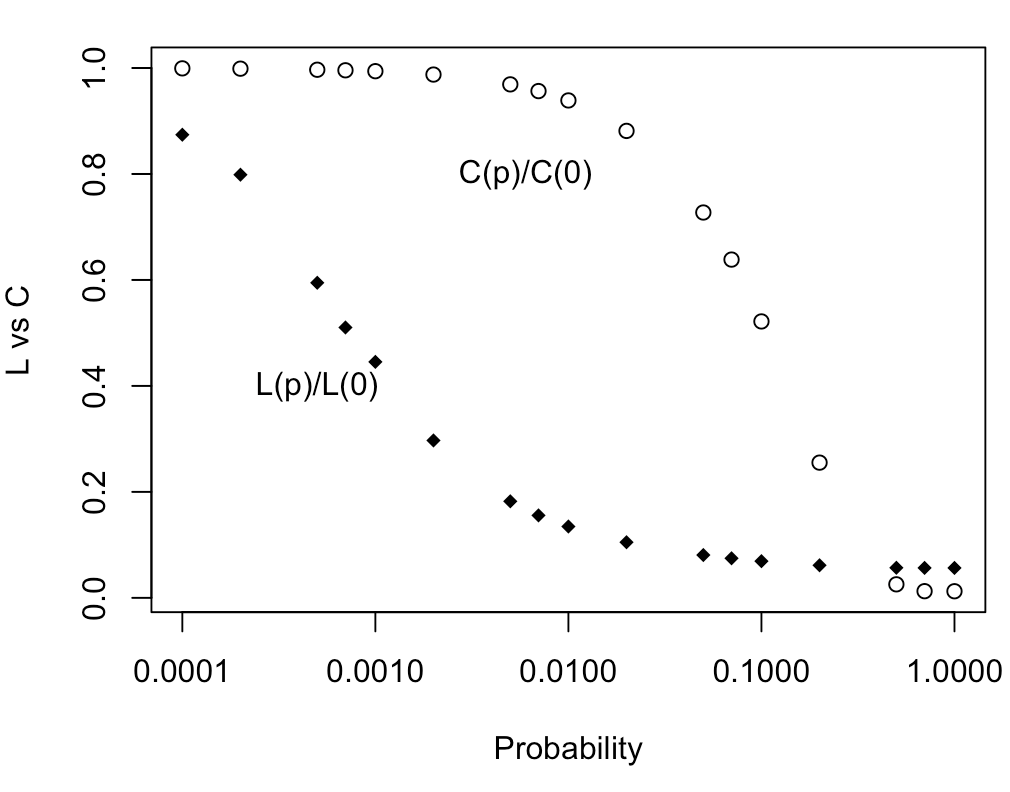
\includegraphics[scale=0.5]{img1.png}\newline
\end{center}

\noindent \underline{ER Network:} \newline


\begin{center}
    

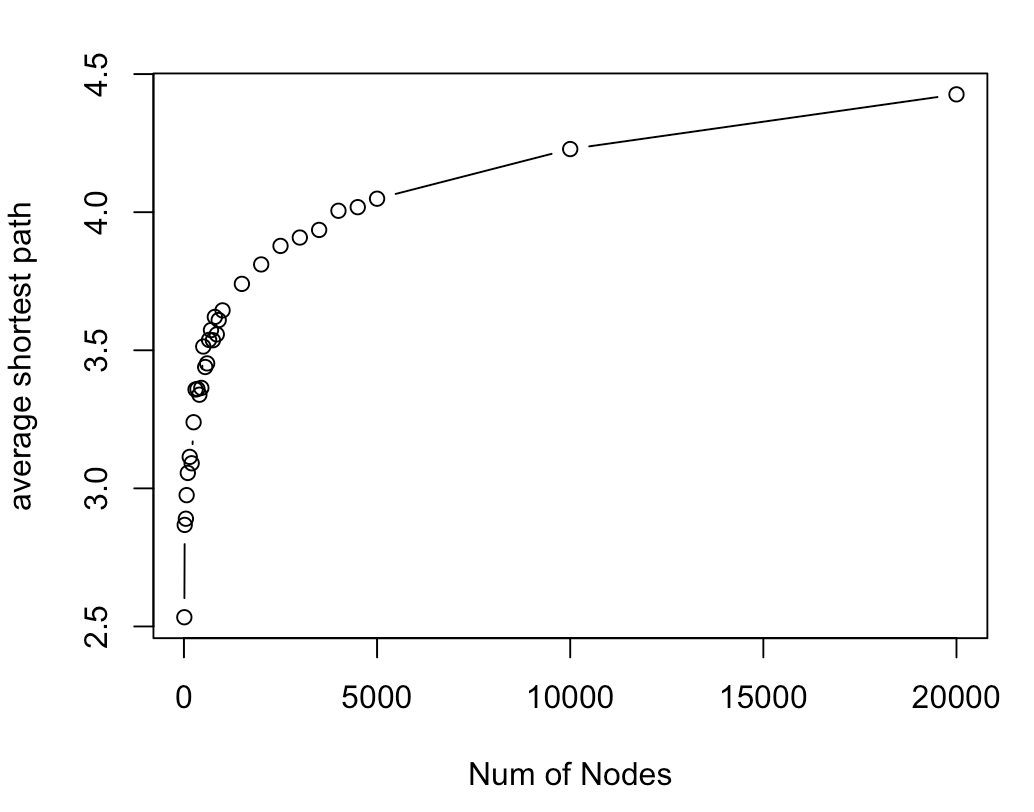
\includegraphics[scale=0.5]{img2.png}\newline
\end{center}


\section{Conclusions}

\noindent \underline{WS Network:} As we can see in table 1, as p (rewiring prob.) increases, the clustering coefficient decreases as well as average shortest path, even though they do this with different rate.\newline 

\noindent The p that we would use to model a real network is something around 0.01 because is in that moment where the network still exhibit a high clustering coefficient but a low average shortest path.\newline

\noindent However we now that WS doesn't have a power-law degree distribution and this is also a property found in real networks.\newline

\noindent \underline{ER Network:} As we can see in table 2, as the number of nodes increase, the avarage shortest path increase but with smaller growth rate as we go up. And even it seems that it is stabilized as the number of nodes reaches 2000. For p (prob. that node i and j are connected), we used: \newline

\[ p= \frac{(1+0.1) * ln\ n}{n} \]\newline

\noindent because we want connected graphs. \newline


\end{document}
